\documentclass[border=2pt,draw]{standalone}
\usepackage{tikz}
\usetikzlibrary{fit,arrows,positioning}
\tikzset{
level/.style={
sibling distance={width("HHHHH$H^{n-2}_{I(n-2)+1}$")+10pt},
level distance=2mm,
line width=.7pt,
},
data/.style={
  minimum width={width("$H^126$")+2pt},
  minimum height={1.1cm},
  inner sep=3 pt,
  outer sep=1,
  rectangle,
  rounded corners=3pt,
  draw,
},
edge from parent/.style={draw=none},
mtedge/.style={grow=down,draw=none,<-, edge from parent/.style={draw}},
pil/.style={
       ->,
       thick,
       shorten <=2pt,
       shorten >=2pt,
},
every node/.style={align=center}
}
\begin{document}

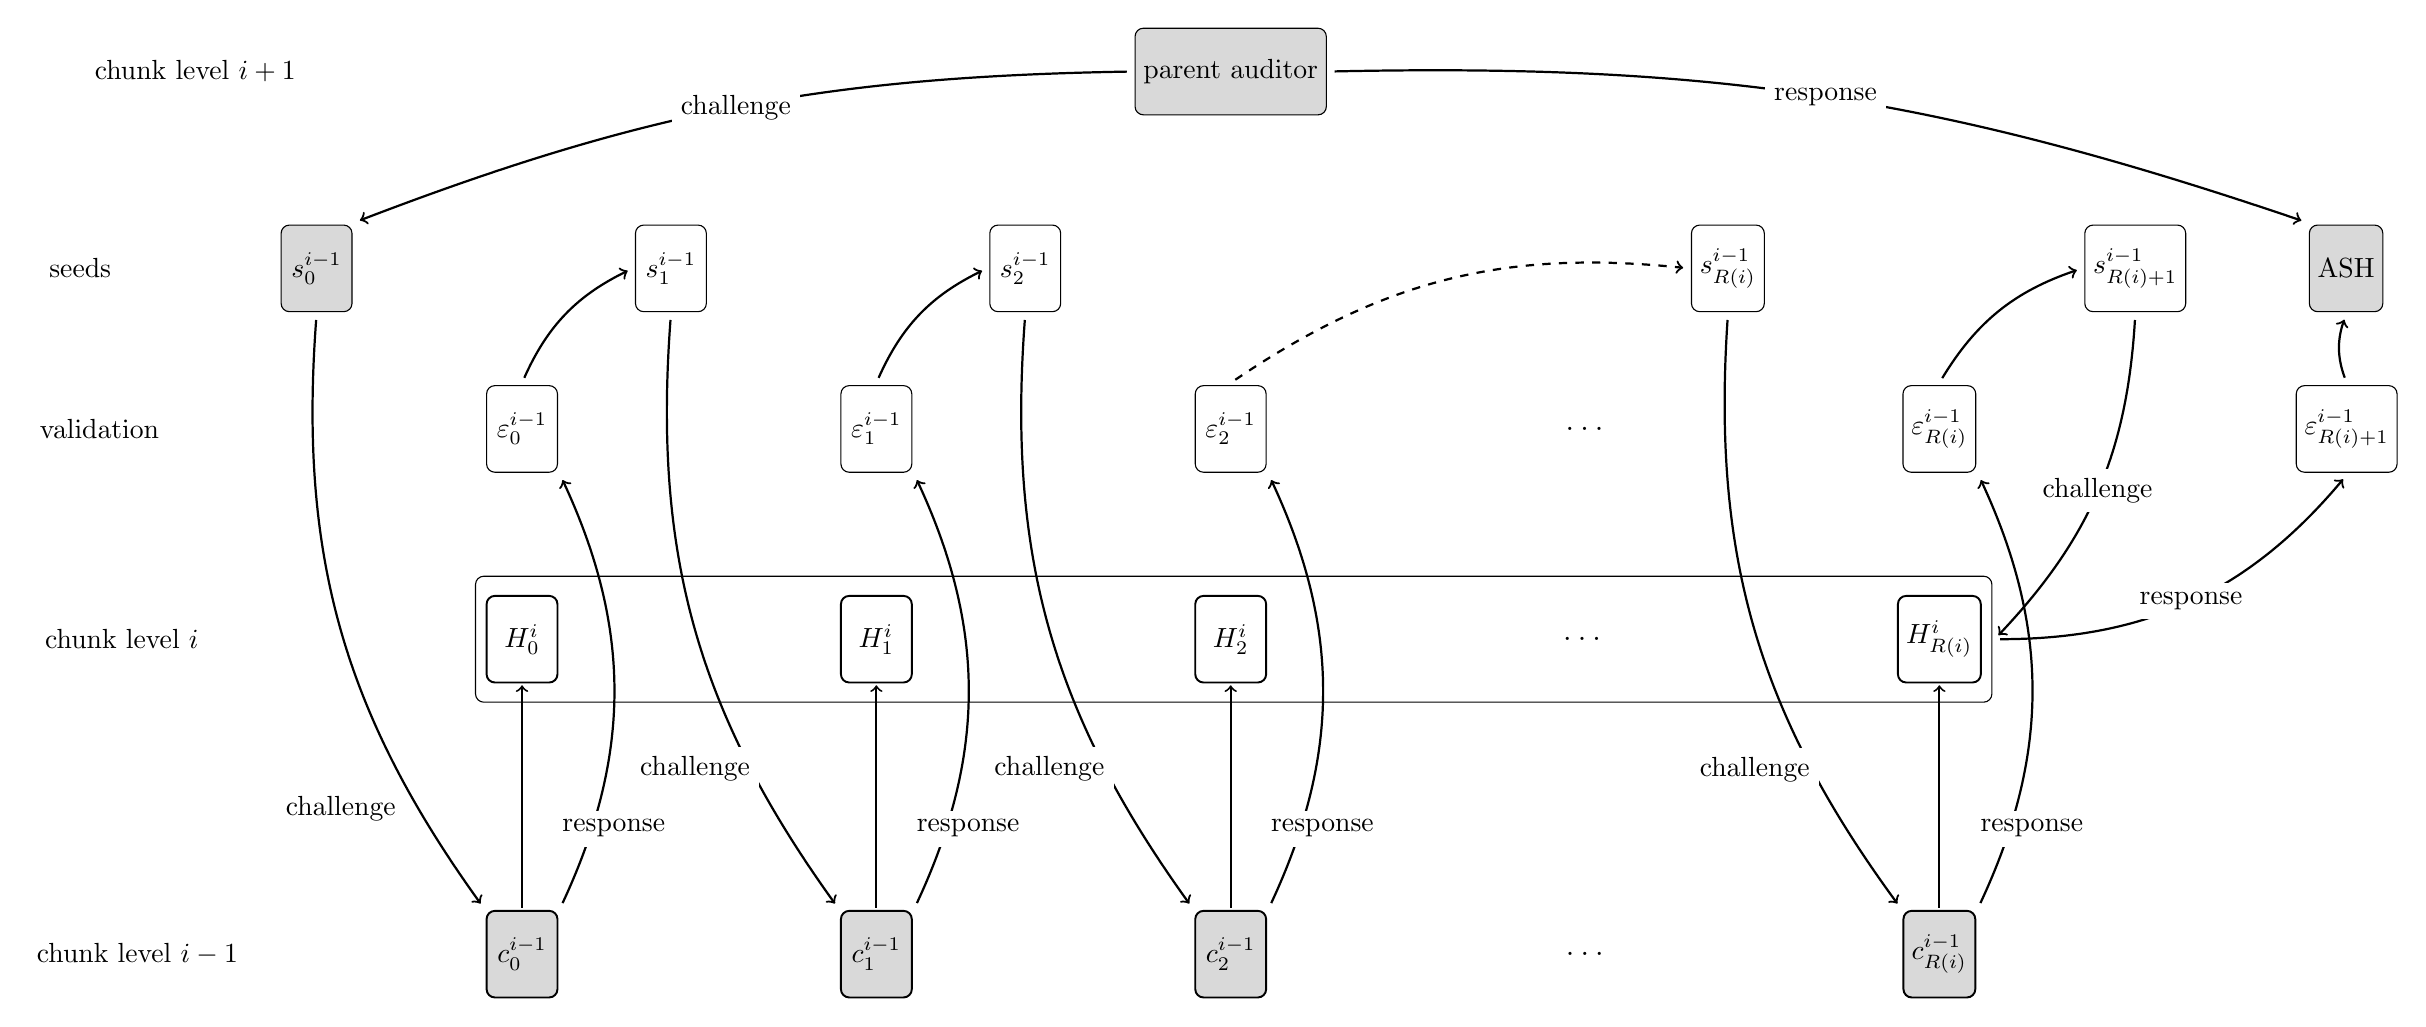
\begin{tikzpicture}[level/.style={sibling distance=45mm, line width=0.7pt, level distance=40mm},
]
\node [draw=none] (root) {}
  child {node [data] (h0) {$H^{i}_{0}$} edge from parent[draw=none]
    child[mtedge] { node[data,fill=gray!30] (c0) {$c^{i-1}_{0}$}}
  }
  child {node [data] (h1) {$H^{i}_{1}$} edge from parent[draw=none]
    child[mtedge] { node[data,fill=gray!30] (c1) {$c^{i-1}_{1}$}}
  }
  child {node [data] (h2) {$H^{i}_{2}$} edge from parent[draw=none]
    child[mtedge] { node[data,fill=gray!30] (c2) {$c^{i-1}_{2}$}}
  }
  child[missing]{node { $c^{i}_{0}$}}
  child {node [data] (hn) {$H^{i}_{R(i)}$} edge from parent[draw=none]
    child[mtedge] { node[data,fill=gray!30] (cn) {$c^{i-1}_{R(i)}$}}
  }
;
\node[left=2cm of h0] (hl0) {};
\node[left=2cm of h1] (hl1) {};
\node[left=2cm of h2] (hl2) {};
\node[left=2cm of hn] (hln) {};


\node[data,above=4cm of hl0,fill=gray!30] (b0) {$s^{i-1}_{0}$};
\node[data,above=4cm of hl1] (b1) {$s^{i-1}_{1}$};
\node[data,above=4cm of hl2] (b2) {$s^{i-1}_{2}$};
\node[data,above=4cm of hln] (bn) {$s^{i-1}_{R(i)}$};
\node[data,right=4cm of bn] (bn1) {$s^{i-1}_{R(i)+1}$};
\node[data,right=1.5cm of bn1,fill=gray!30] (bn2) {ASH};
% \node[data,right=1cm] (bi) {$\varepsilon^{i-1}_{1}$};
\node[data,above=1.5cm of h0] (e0) {$\varepsilon^{i-1}_{0}$};
\node[data,above=1.5cm of h1] (e1) {$\varepsilon^{i-1}_{1}$};
\node[data,above=1.5cm of h2] (e2) {$\varepsilon^{i-1}_{2}$};
\node[data,above=1.5cm of hn] (en) {$\varepsilon^{i-1}_{R(i)}$};
\node[data,right=4cm of en] (en1) {$\varepsilon^{i-1}_{R(i)+1}$};

\node[data,above=2.5cm of root,fill=gray!30] (au)  {parent auditor};
\node[left=2cm of b0]{seeds};
\node[left=4cm of e0]{validation};
\node[left=3.5cm of h0]{chunk level $i$};
\node[left=3cm of c0]{chunk level $i-1$};
\node[left=10.5cm of au]{chunk level $i+1$};

\path (h2) -- (hn) node [midway,font=\large] {$\ldots$};
\path (c2) -- (cn) node [midway,font=\large] {$\ldots$};
\path (e2) -- (en) node [midway,font=\large] {$\ldots$};

\node[data, minimum height=1.6cm, fit=(h0) (hn)] (c) {}
  (b0.south) edge[pil, ->, bend right=20] node[fill=white,below=2cm] (ch0) {challenge} (c0.north west)
  (c0.north east) edge[pil, ->, bend right=25] node[fill=white,below=1.5cm] (r0) {response} (e0.south east)
  (e0.north) edge[pil, ->, bend left=20] node[fill=white,above=10pt] {} (b1.west)
  (b1.south) edge[pil, ->, bend right=20] node[fill=white,below=1.5cm] (ch1) {challenge} (c1.north west)
  (c1.north east) edge[pil, ->, bend right=25] node[fill=white,below=1.5cm] (r1) {response} (e1.south east)
  (e1.north) edge[pil, ->, bend left=20] node[fill=white,above=10pt] {} (b2.west)
  (b2.south) edge[pil, ->, bend right=20] node[fill=white,below=1.5cm] (ch2) {challenge} (c2.north west)
  (c2.north east) edge[pil, ->, bend right=25] node[fill=white,below=1.5cm] (r2) {response} (e2.south east)
  (e2.north) edge[pil,dashed, ->, bend left=20] node[fill=white,above=10pt] {} (bn.west)
(bn.south) edge[pil, ->, bend right=20] node[fill=white,below=1.5cm] (chn) {challenge} (cn.north west)
  (cn.north east) edge[pil, ->, bend right=25] node[fill=white,below=1.5cm] (rn) {response} (en.south east)
  (en.north) edge[pil, ->, bend left=20] node {} (bn1.west)
(bn1.south) edge[pil, ->, bend left=20] node[fill=white] (chn) {challenge} (c.east)
  (c.east) edge[pil, ->, bend right=25] node[fill=white] (rn) {response} (en1.south)
  (en1.north) edge[pil, ->, bend left=20] node {} (bn2.south)
  (au.west) edge[pil, ->, bend right=10] node[fill=white] {challenge} (b0.north east)
  (au.east) edge[pil, ->, bend left=10] node[fill=white] {response} (bn2.north west)
;
\end{tikzpicture}

\end{document}
